%%%%%%%%%%%%%%%%%%%%%%%%%%%%%%%%%%%%%%%%%%%%%%%%%%%%%%%%%%%%%%%%%%%%%%%%%%%%%%%%
%%%%%%%%%%%%%%%%%%%%%%%%%%%%%%%%%%%%%%%%%%%%%%%%%%%%%%%%%%%%%%%%%%%%%%%%%%%%%%%%
%%%%%%%%%%%%%%%%%%%%%%%%%%%%%%%%%%%%%%%%%%%%%%%%%%%%%%%%%%%%%%%%%%%%%%%%%%%%%%%%
%%%%%%%%%%%%%%%%%%%%%%%%%%%%%%%%%%%%%%%%%%%%%%%%%%%%%%%%%%%%%%%%%%%%%%%%%%%%%%%%
\chapter{Asservissements des systèmes linéaires\label{chap-asservis}}
%%%%%%%%%%%%%%%%%%%%%%%%%%%%%%%%%%%%%%%%%%%%%%%%%%%%%%%%%%%%%%%%%%%%%%%%%%%%%%%%
%%%%%%%%%%%%%%%%%%%%%%%%%%%%%%%%%%%%%%%%%%%%%%%%%%%%%%%%%%%%%%%%%%%%%%%%%%%%%%%%
%%%%%%%%%%%%%%%%%%%%%%%%%%%%%%%%%%%%%%%%%%%%%%%%%%%%%%%%%%%%%%%%%%%%%%%%%%%%%%%%
%%%%%%%%%%%%%%%%%%%%%%%%%%%%%%%%%%%%%%%%%%%%%%%%%%%%%%%%%%%%%%%%%%%%%%%%%%%%%%%%
\minitoc
\newpage
%%%%%%%%%%%%%%%%%%%%%%%%%%%%%%%%%%%%%%%%%%%%%%%%%%%%%%%%%%%%%%%%%%%%%%%%%%%%%%%%
%%%%%%%%%%%%%%%%%%%%%%%%%%%%%%%%%%%%%%%%%%%%%%%%%%%%%%%%%%%%%%%%%%%%%%%%%%%%%%%%
%%%%%%%%%%%%%%%%%%%%%%%%%%%%%%%%%%%%%%%%%%%%%%%%%%%%%%%%%%%%%%%%%%%%%%%%%%%%%%%%
\section{Introduction}
%%%%%%%%%%%%%%%%%%%%%%%%%%%%%%%%%%%%%%%%%%%%%%%%%%%%%%%%%%%%%%%%%%%%%%%%%%%%%%%%
%%%%%%%%%%%%%%%%%%%%%%%%%%%%%%%%%%%%%%%%%%%%%%%%%%%%%%%%%%%%%%%%%%%%%%%%%%%%%%%%
%%%%%%%%%%%%%%%%%%%%%%%%%%%%%%%%%%%%%%%%%%%%%%%%%%%%%%%%%%%%%%%%%%%%%%%%%%%%%%%%

\begin{figure}[!h]
\centering
%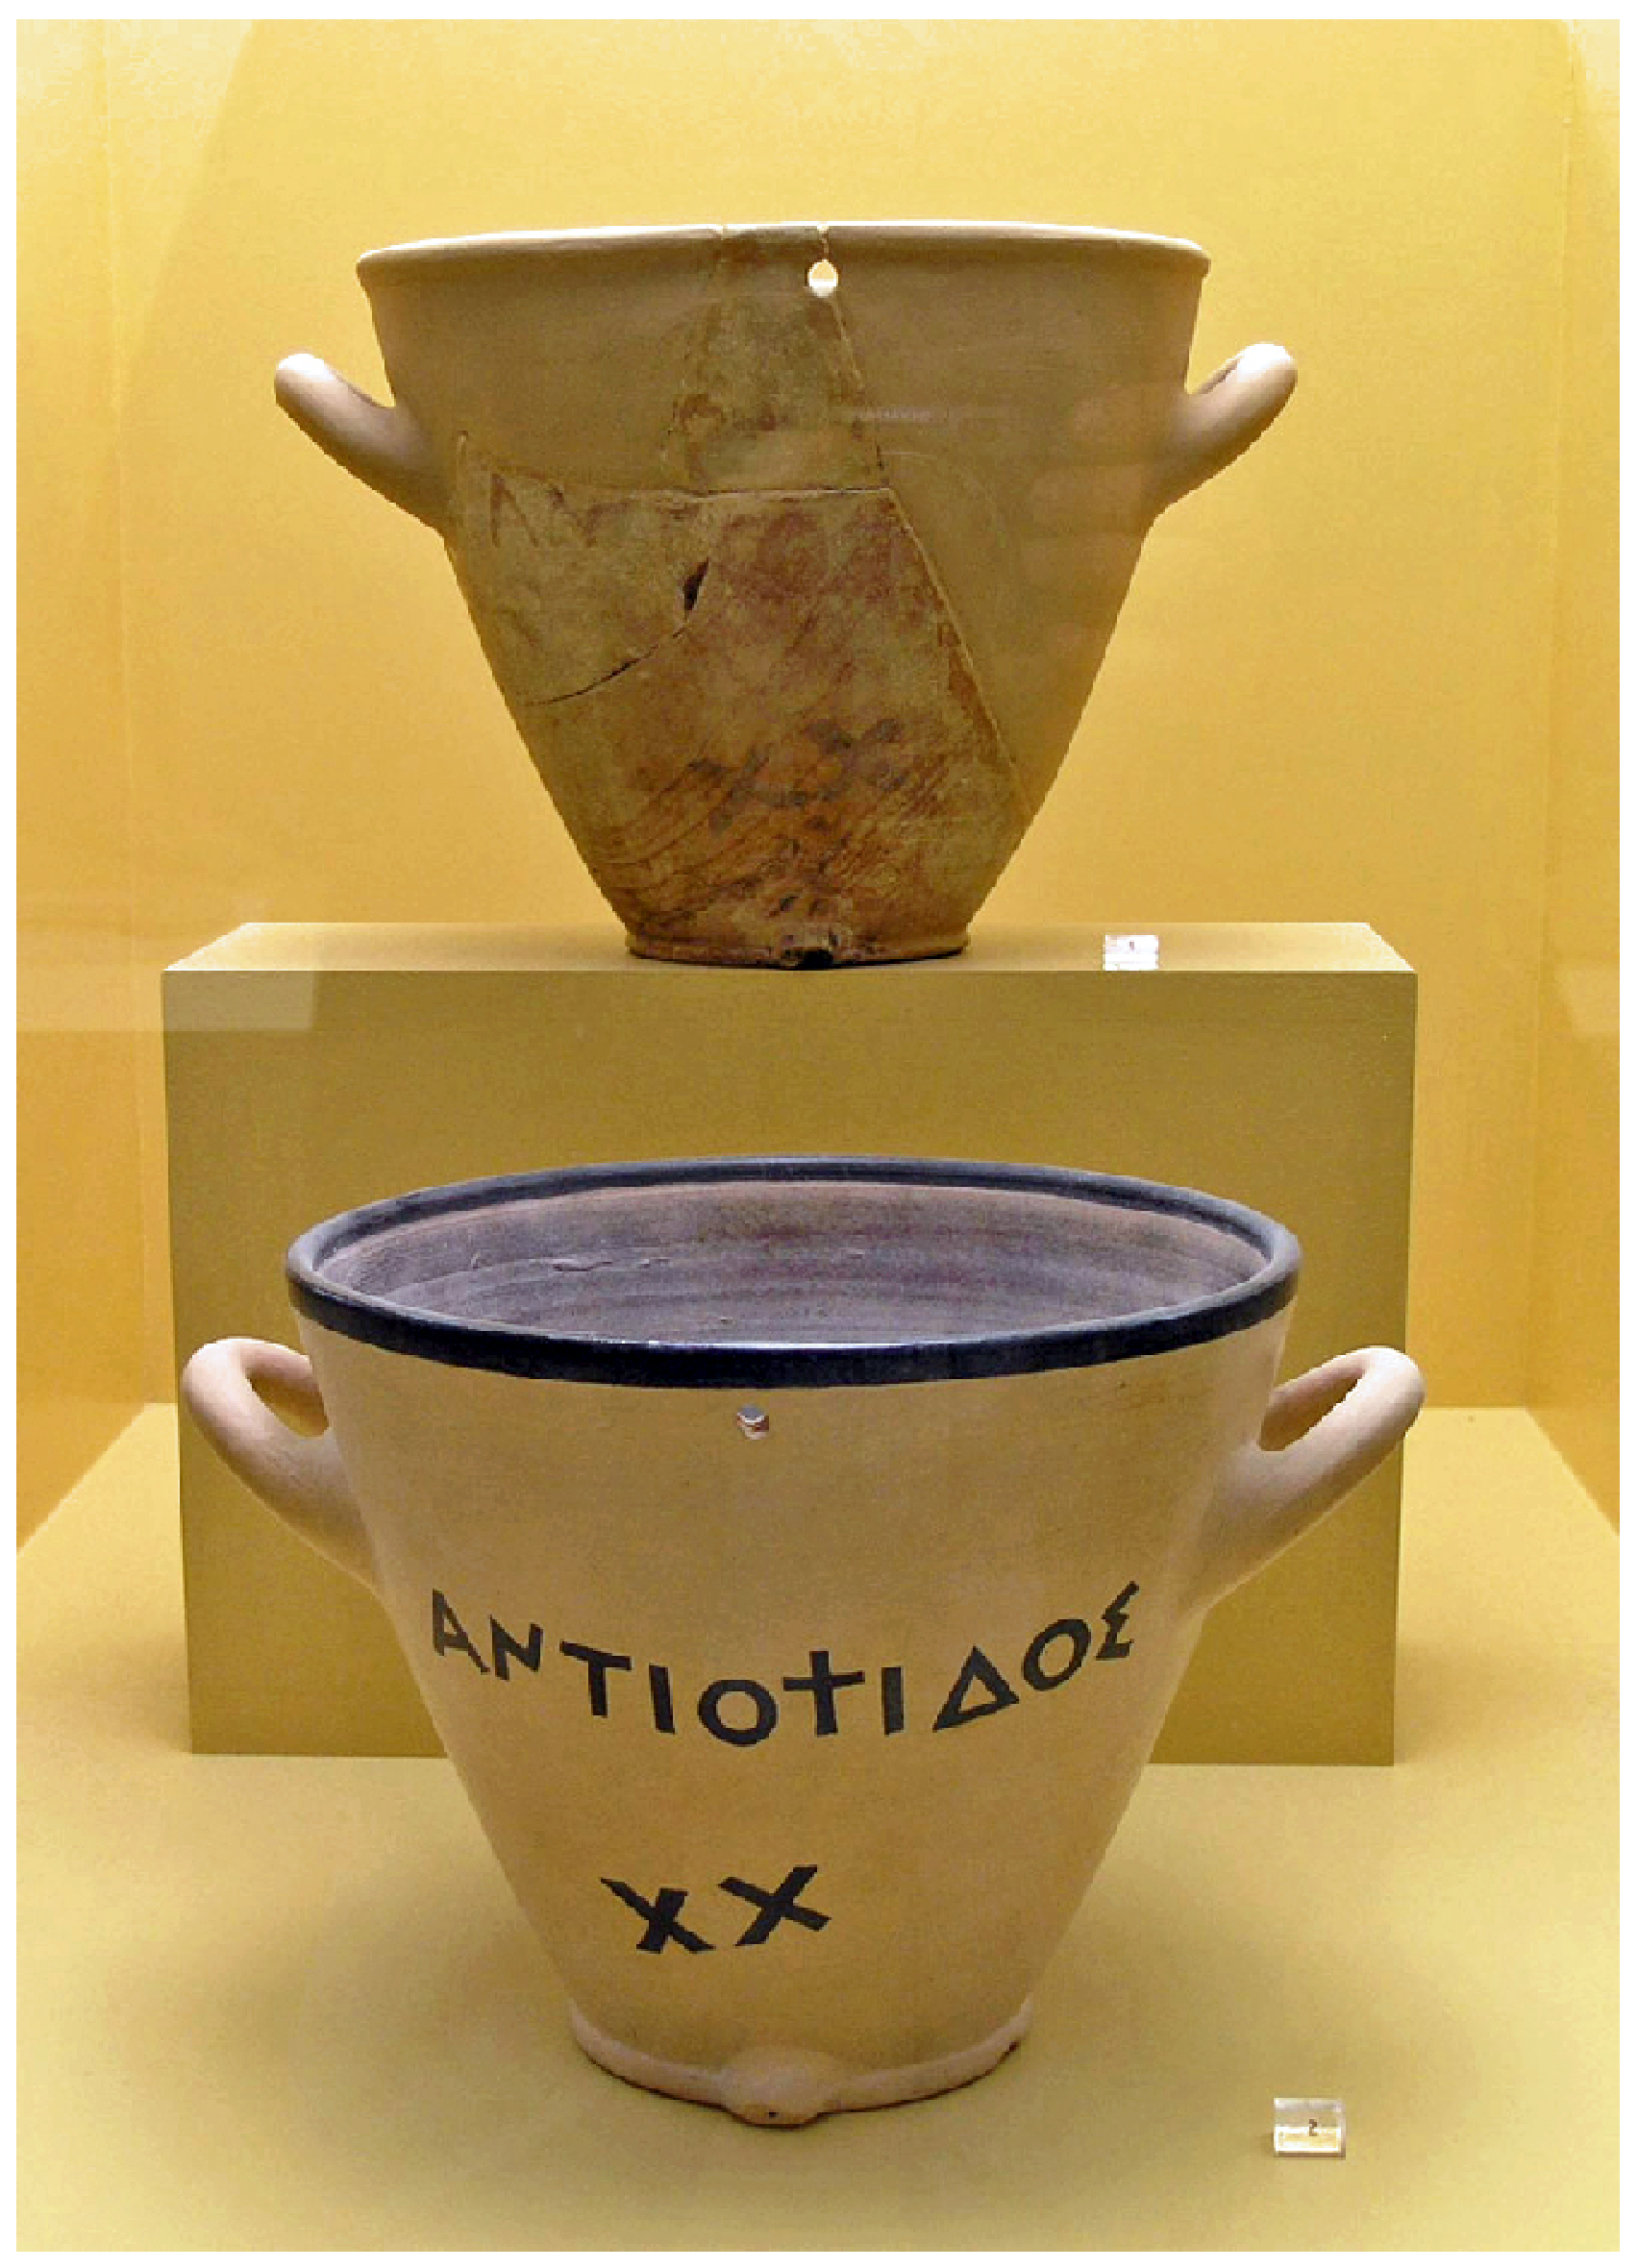
\includegraphics[width=0.45\linewidth,height=10cm]{fig/AGMA_Clepsydre_m.eps}
%\label{fig-clep}
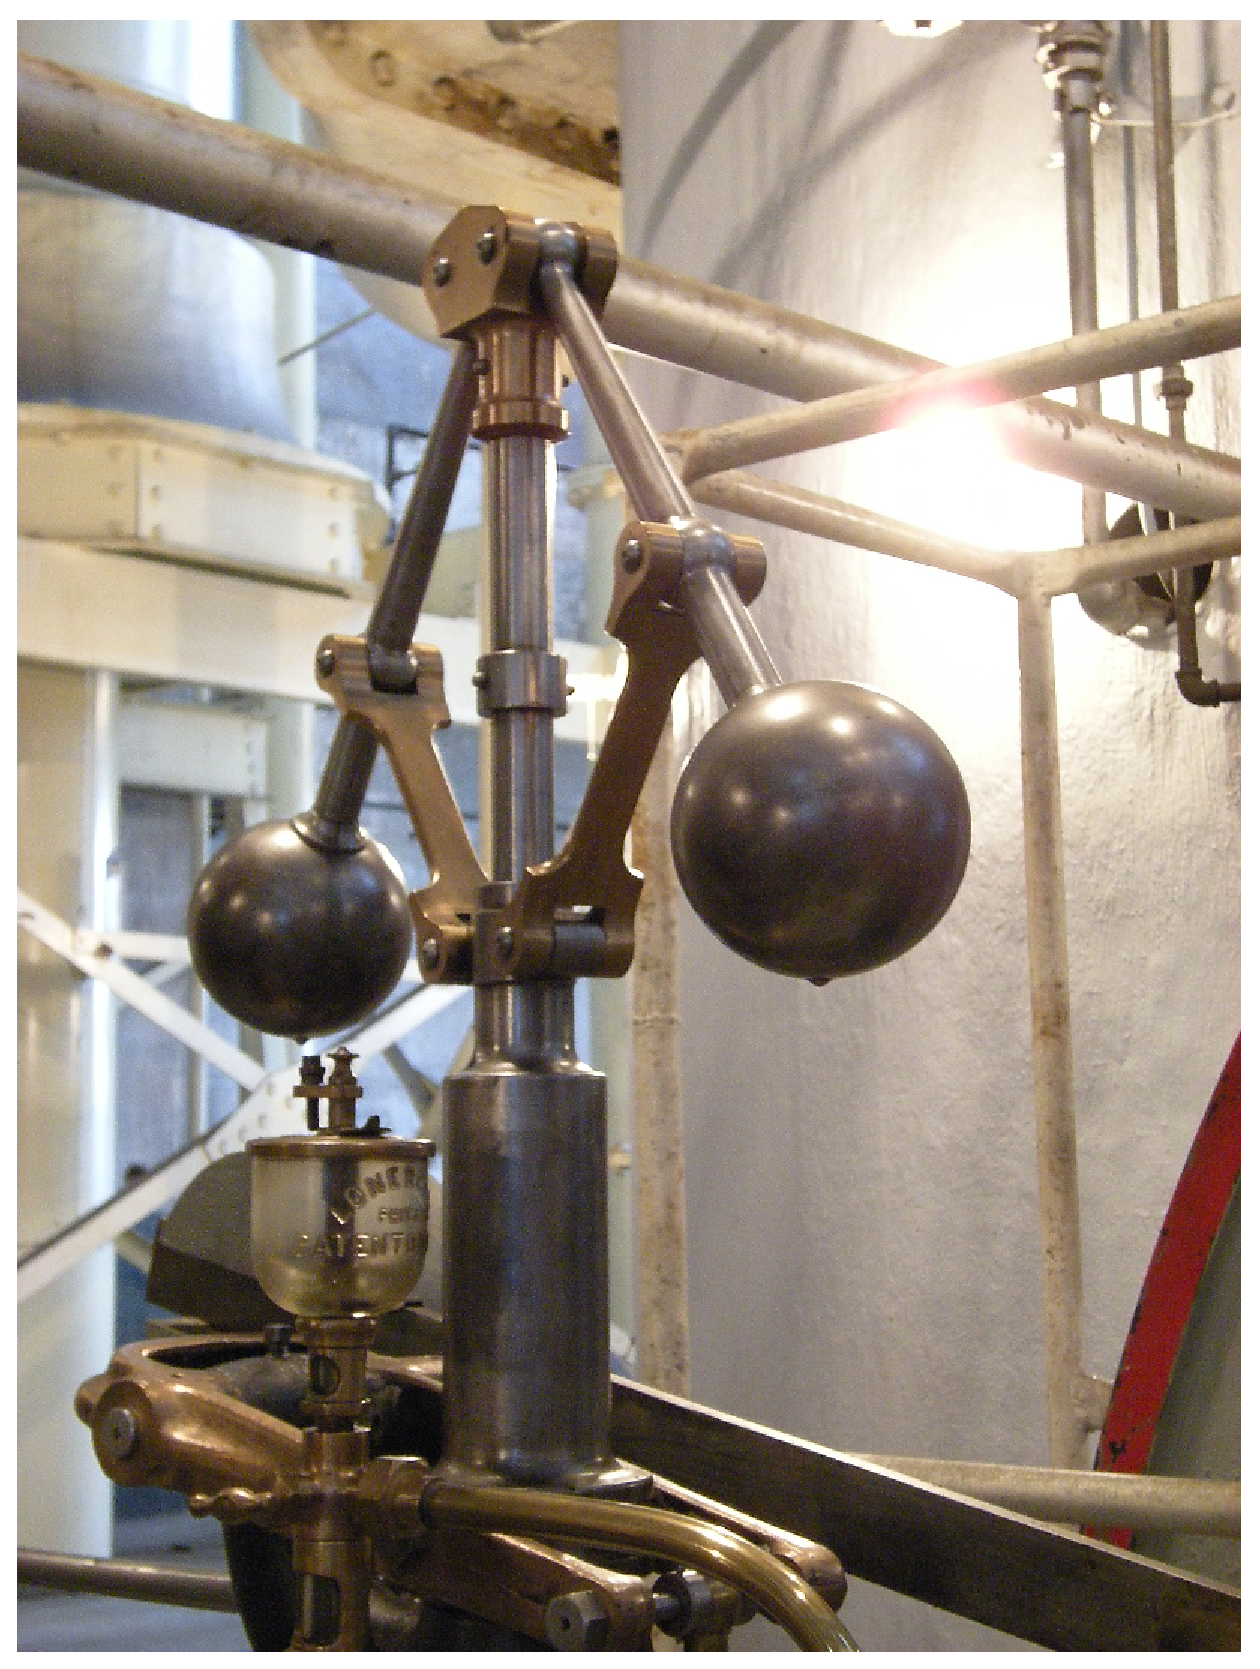
\includegraphics[width=0.45\linewidth,height=10cm]
{fig/Georgetown_PowerPlant_Museum_m.eps}
%\label{fig-watt}
%\caption{Exemples historiques de régulateur : 
%(gauche) Clepsydre athénienne (d'après \cite{clep}) 
%(droite) Régulateur de vitesse de Watt (d'après \cite{watt})\label{fig-hist}}
\caption{Exemple historique de régulateur : Régulateur 
de vitesse de Watt (d'après \cite{watt})\label{fig-hist}}
\end{figure}

Les chapitres précédents nous ont permis de caractériser, modéliser et
analyser la réponse temporelle des systèmes linéaires.
Nous allons maintenant aborder la possibilité du \textbf{contrôle} de ces 
systèmes par l'intermédiaire de l'\textbf{asservissement} et de 
\textbf{régulation}. 
L'idée sous-jacente est de permettre le contrôle automatique d'un système
sans l'intervention d'un opérateur humain dans l'établissement d'une commande
d'un système. 

La figure~\ref{fig-hist} montre un exemple historique de régulateur de 
vitesse ( également connu comme le régulateur à boules de Watt). 
La particularité de ce régulateur est d'avoir était utilisé dans l'industrie
du 18ème siècle bien avant les premières avancées théoriques dans le domaine 
de l'automatique. Dans le contexte des premières machines à vapeurs, 
il était important de contrôler la vitesse angulaire des turbines à vapeur. 
Le mécanisme de Watt permet avec un dispositif de retroaction d'agir sur la 
valve d'arrivée de la vapeur en fonction de la vitesse de l'axe de la turbine.

\clearpage
Jusqu'à présent nous nous sommes intéressés à l'étude de système 
linéaire \og isolé\fg (de fonction de transfert $H(p)$) 
qui pour une entrée $E(p)$, élaborait une sortie $S(p)$\footnote{Nous
continuerons, dans ce chapitre et les suivants, de représenter 
les signaux et systèmes linéaires dans le domaine de Laplace. Une approche temporelle
sera introduite au~\cref{chap-repreEtat}}.
Dans le contexte du contrôle de ces systèmes l'entrée est appelée 
\textbf{consigne} et la sortie est la \textbf{réponse}. Le problème de 
\textbf{l'asservissement} consiste à faire en sorte que la réponse suive 
la consigne au cours du temps.

La \textbf{régulation} est un cas particulier d'asservissement, consistant
à contrôler la sortie d'un système pour une consigne fixe quelque soit 
les perturbations auxquelles serait soumis le système.

%%%%%%%%%%%%%%%%%%%%%%%%%%%%%%%%%%%%%%%%%%%%%%%%%%%%%%%%%%%%%%%%%%%%%%%%%%%%%%%%
%   Nom des noeuds
%                                      
%                                      
%   E ---- a ---- S
%
% E : entrée
% a : système 
% S : sortie
%%%%%%%%%%%%%%%%%%%%%%%%%%%%%%%%%%%%%%%%%%%%%%%%%%%%%%%%%%%%%%%%%%%%%%%%%%%%%%%%
\begin{center}
\tikzsetnextfilename{sb_bloc0-chap5-ext}
\begin{tikzpicture}
    \sbEntree{E}
    \sbBloc[3]{a}{$H(p)$}{E}
    \sbRelier[$E(p)$]{E}{a}
    \sbSortie[3]{S}{a}
    \sbRelier[$S(p)$]{a}{S}
\end{tikzpicture}
\end{center}

Nous avons pu caractériser la sortie en fonction de différentes 
critères de performances: rapidité, précision, stabilité et dépassement\ldots
pour différents systèmes linéaires modèles (c.f~\cref{chap-model}). 
La question est de savoir comment agir sur le 
signal $E(p)$ pour contrôler la sortie $S(p)$ en fonction de 
ces exigences de performances choisis initialement.

Il existe deux approches pour élaborer la \textbf{commande} 
d'un système linéaire :% soit en boucle ouverte soit en boucle fermée.

\begin{itemize}
    \item En \textbf{boucle ouverte}: on place un correcteur $C(p)$
          en amont du système pour élaborer 
          sa commande (notée $U(p)$).
          Remarquons que la consigne est maintenant
          l'entrée du correcteur.

%%%%%%%%%%%%%%%%%%%%%%%%%%%%%%%%%%%%%%%%%%%%%%%%%%%%%%%%%%%%%%%%%%%%%%%%%%%%%%%%
%   Nom des noeuds
%                                      
%                                      
%   E ---- a ---- b ---- S
%
% E : entrée
% a : correcteur 
% b : système 
% S : sortie
%%%%%%%%%%%%%%%%%%%%%%%%%%%%%%%%%%%%%%%%%%%%%%%%%%%%%%%%%%%%%%%%%%%%%%%%%%%%%%%%
\begin{center}
\tikzsetnextfilename{sb_bloc1-chap5-ext}
\begin{tikzpicture}
    \sbEntree{E}
    \sbBloc[3]{a}{$C(p)$}{E}
    \sbRelier[$E(p)$]{E}{a}
    \sbBloc[3]{b}{$H(p)$}{a}
    \sbRelier[$U(p)$]{a}{b}
    \sbSortie[3]{S}{b}
    \sbRelier[$S(p)$]{b}{S}
    \node[yshift=-0.8em] at (a.south) {\small Correcteur};
    \node[yshift=-0.8em] at (b.south) {\small Système};
\end{tikzpicture}
\end{center}

    \item En \textbf{boucle fermée}: le principe consiste à récupérer 
          le signal de sortie pour ajuster le signal de commande. 
          Pour celà, on place le système (corrigée ou non) dans une 
          boucle de contre-réaction (négative). 
          Les relations entre la sortie et la consigne dans une telle 
          boucle ont été largement étudiées au \cref{chap-schemabloc}.

%%%%%%%%%%%%%%%%%%%%%%%%%%%%%%%%%%%%%%%%%%%%%%%%%%%%%%%%%%%%%%%%%%%%%%%%%%%%%%%%
%   Nom des noeuds
%                                      
%                                      
%   E ---- a ---- b ---- c ---- S
%          |                    |
%          |                    |
%          ---------------------
%
% E : entrée
% a : comparateur
% b : correcteur
% c : système
% S : sortie
%%%%%%%%%%%%%%%%%%%%%%%%%%%%%%%%%%%%%%%%%%%%%%%%%%%%%%%%%%%%%%%%%%%%%%%%%%%%%%%%
\begin{center}
\tikzsetnextfilename{sb_bloc2-chap5-ext}
\begin{tikzpicture}
    \sbEntree{E}
    \sbComp{a}{E}
    \sbRelier[$E(p)$]{E}{a}
    \sbBloc[3]{b}{$C(p)$}{a}
    \sbRelier[$\epsilon(p)$]{a}{b}
    \sbBloc[3]{c}{$H(p)$}{b}
    \sbRelier[$U(p)$]{b}{c}
    \sbSortie[3]{S}{c}
    \sbRelier[$S(p)$]{c}{S}
    \sbRenvoi{c-S}{a}{}
    \node[yshift=-0.8em] at (b.south) {\small Correcteur};
    \node[yshift=-0.8em] at (c.south) {\small Système};
\end{tikzpicture}
\end{center}
          Le signal correspondant à la différence entre la consigne
          et la réponse globale du système en boucle fermée est
          appelée l'\textbf{écart} $\epsilon(p)$.
\end{itemize}

La rétroaction\footnote{\emph{feedback} (en anglais)} est
devenu incontournable dans les applications industrielles                                                                     
et technologiques.
Par abus de langage c'est le système en boucle fermée
que l'on nomme asservissement. Cependant, la 
définition précédente de l'asservissement s'applique très bien dans 
le cas de la boucle ouverte.

\clearpage
%%%%%%%%%%%%%%%%%%%%%%%%%%%%%%%%%%%%%%%%%%%%%%%%%%%%%%%%%%%%%%%%%%%%%%%%%%%%%%%%
%%%%%%%%%%%%%%%%%%%%%%%%%%%%%%%%%%%%%%%%%%%%%%%%%%%%%%%%%%%%%%%%%%%%%%%%%%%%%%%%
%%%%%%%%%%%%%%%%%%%%%%%%%%%%%%%%%%%%%%%%%%%%%%%%%%%%%%%%%%%%%%%%%%%%%%%%%%%%%%%%
\section{Organisation d'un asservissement}
%%%%%%%%%%%%%%%%%%%%%%%%%%%%%%%%%%%%%%%%%%%%%%%%%%%%%%%%%%%%%%%%%%%%%%%%%%%%%%%%
%%%%%%%%%%%%%%%%%%%%%%%%%%%%%%%%%%%%%%%%%%%%%%%%%%%%%%%%%%%%%%%%%%%%%%%%%%%%%%%%
%%%%%%%%%%%%%%%%%%%%%%%%%%%%%%%%%%%%%%%%%%%%%%%%%%%%%%%%%%%%%%%%%%%%%%%%%%%%%%%%

%%%%%%%%%%%%%%%%%%%%%%%%%%%%%%%%%%%%%%%%%%%%%%%%%%%%%%%%%%%%%%%%%%%%%%%%%%%%%%%%
%%%%%%%%%%%%%%%%%%%%%%%%%%%%%%%%%%%%%%%%%%%%%%%%%%%%%%%%%%%%%%%%%%%%%%%%%%%%%%%%
\subsection{Schémas fonctionnels associés aux systèmes asservis}
%%%%%%%%%%%%%%%%%%%%%%%%%%%%%%%%%%%%%%%%%%%%%%%%%%%%%%%%%%%%%%%%%%%%%%%%%%%%%%%%
%%%%%%%%%%%%%%%%%%%%%%%%%%%%%%%%%%%%%%%%%%%%%%%%%%%%%%%%%%%%%%%%%%%%%%%%%%%%%%%%

Classiquement, un asservissement se représente par le schéma fonctionnel de 
la figure (\cref{fig-reg}). Celui-ci comporte en générale un \textbf{régulateur}
permettant de comparer l'image de la sortie obtenue par un capteur à la consigne.
Ce régulateur est en générale accompagné d'un \textbf{correcteur} permettant de corriger
la boucle ouverte du système linéaire.

\begin{figure}[!h]
\centering
%%%%%%%%%%%%%%%%%%%%%%%%%%%%%%%%%%%%%%%%%%%%%%%%%%%%%%%%%%%%%%%%%%%%%%%%%%%%%%%%
%   Nom des noeuds
%                                      
%   E ---- a ---- b ---- c ---- S
%          |                |
%          |                |
%            ---- d ------- 
% E : entrée
% a : comparateur
% b : correcteur
% c : système
% S : sortie
% d : capteur
% r : noeud décalé pour le retour
%%%%%%%%%%%%%%%%%%%%%%%%%%%%%%%%%%%%%%%%%%%%%%%%%%%%%%%%%%%%%%%%%%%%%%%%%%%%%%%%
%avec cadre régulateur
\tikzsetnextfilename{reg_1-chap5-ext}
\begin{tikzpicture}
    \sbEntree{E}
    \sbComp{a}{E}
    \sbRelier[$E(p)$]{E}{a}           % entree
    \sbBloc[3]{b}{$C(p)$}{a}
    \sbRelier[$\epsilon(p)$]{a}{b}    % ecart
    \sbBloc[4.2]{c}{$H(p)$}{b}
    \sbRelier[$U(p)$]{b}{c}           % commande
    \sbSortie[4]{S}{c}
    \sbRelier{c}{S}
    \sbNomLien[0.8]{S}{$S(p)$}
    \sbDecaleNoeudy[7]{b-c}{r}
    \sbBlocr[-1.6]{d}{$G(p)$}{r}
    \sbRelieryx{c-S}{d}              
    \sbRelierxy[$M(p)$]{d}{a}         % mesure (image de S)
    \node[yshift=-0.8em] at (b.south) {\small Correcteur};
    \node[yshift=-0.8em] at (c.south) {\small Système};
    \node[yshift=-0.8em] at (d.south) {\small Capteur};
    \draw[dvtb] (1.05,-1.65) rectangle node[blue,above,yshift=4em] {\textbf{Régulateur}} (4.65,0.9);
    \node[yshift=-0.8em,xshift=0.5em] at (E.south) {\small Consigne};
    \node[yshift=-0.8em] at (S.south) {\small Sortie};
\end{tikzpicture}
\caption{Schéma fonctionnel classique de l'asservissement d'un système 
         présentant un correcteur et un capteur. (c.f~\cref{tab-asser})
         \label{fig-reg}}
\end{figure}


La \textbf{mesure} $M(p)$ est l'image de la sortie par l'intermédiaire
du capteur. Il est alors en générale nécessaire d'adapter la consigne pour
que l'écart $\epsilon(p)$ soit représentatif de l'écart entre la consigne
et la sortie et non de son image. Ainsi, on retrouvera très souvent 
un \textbf{adaptateur} permmettant d'obtenir l'image de la consigne.
Le procédé/système peux nécéssité d'un \textbf{actionneur} qui agit en 
transmettant/convertissant l'énergie nécéssaire à son action. 
La~\cref{fig-reg2} présente une forme augmentée de schéma fonctionnel
présentant ces nouveaux constituants.


%%%%%%%%%%%%%%%%%%%%%%%%%%%%%%%%%%%%%%%%%%%%%%%%%%%%%%%%%%%%%%%%%%%%%%%%%%%%%%%%
%   Nom des noeuds
%                                      
%                                      
%   E ---- a ---- b ---- c ---- d ---- e ---- S
%                 |                           |
%                 |                           |
%                  --------- f -----------
% E : entrée
% a : adaptateur 
% b : comparateur
% c : correcteur
% d : actionneur
% e : système
% S : sortie
% f : capteur
% r : noeud décalé pour le retour
%%%%%%%%%%%%%%%%%%%%%%%%%%%%%%%%%%%%%%%%%%%%%%%%%%%%%%%%%%%%%%%%%%%%%%%%%%%%%%%%
\begin{figure}[!h]
\centering
\tikzsetnextfilename{reg_2-chap5-ext}
\begin{tikzpicture}
    \sbEntree{E}
    \sbBloc[3]{a}{$A_d(p)$}{E}
    \sbRelier[$E(p)$]{E}{a}
    \sbComp{b}{a}
    \sbRelier{a}{b}
    \sbBloc[3]{c}{$C(p)$}{b}
    \sbRelier[$\epsilon(p)$]{b}{c}
    \sbBloc[3]{d}{$A_c(p)$}{c}
    \sbRelier{c}{d}
    \sbBloc[3]{e}{$H(p)$}{d}
    \sbRelier[$U(p)$]{d}{e}
    \sbSortie[4]{S}{e}
    \sbRelier{e}{S}
    \sbDecaleNoeudy[5]{d}{r}
    \sbBlocr[-1.6]{f}{$G(p)$}{r}
    \sbRelieryx{e-S}{f}              
    \sbRelierxy[$M(p)$]{f}{b}        % Mesure
    \sbNomLien[0.8]{S}{$S(p)$}
    \node[yshift=-0.8em] at (a.south) {\small Adaptateur};
    \node[yshift=-0.8em] at (c.south) {\small Correcteur};
    \node[yshift=-0.8em] at (d.south) {\small Actionneur};
    \node[yshift=-0.8em] at (e.south) {\small Système};
    \node[yshift=-0.8em] at (f.south) {\small Capteur};
    \node[yshift=-0.8em,xshift=0.5em] at (E.south) {\small Consigne};
    \node[yshift=-0.8em] at (S.south) {\small Sortie};
\end{tikzpicture}
\caption{Schéma fonctionnel de l'asservissement d'un système 
         présentant un adaptateur et actionneur. (c.f~\cref{tab-asser})
         \label{fig-reg2}}
\end{figure}

\subsection{Présence d'une perturbation : la régulation}

%%%%%%%%%%%%%%%%%%%%%%%%%%%%%%%%%%%%%%%%%%%%%%%%%%%%%%%%%%%%%%%%%%%%%%%%%%%%%%%%
%   Nom des noeuds
%                        P             
%                        |             
%                        |              
%   E ---- a ---- b ---- c ---- d ---- S
%          |                           |
%          |                           |
%           ------------ e ------------ 
%                        
%                        
% E : entrée
% a : comparateur/régulateur
% b : correcteur 
% c : sommateur (perturbation)
% d : système 
% e : capteur
% P : noeud décalé pour la perturbation
% S : sortie
% r : noeud décalé pour le retour
%%%%%%%%%%%%%%%%%%%%%%%%%%%%%%%%%%%%%%%%%%%%%%%%%%%%%%%%%%%%%%%%%%%%%%%%%%%%%%%%
\begin{figure}[!h]
    \centering
    \tikzsetnextfilename{pert-chap5-ext}
    \begin{tikzpicture}
    \sbEntree{E}
    \sbComp[4.5]{a}{E}
    \sbRelier[$E(p)$]{E}{a}
    \sbBloc[3]{b}{$C(p)$}{a}
    \sbRelier[$\epsilon(p)$]{a}{b}
    \sbCompSum[5.0]{c}{b}{+}{}{+}{}
    \sbRelier[$U(p)$]{b}{c}
    \sbBloc[3]{d}{$H(p)$}{c}
    \sbRelier{c}{d}
    \sbSortie[6]{S}{d}
    \sbRelier[$S(p)$]{d}{S}
    \sbDecaleNoeudy{c}{r}
    \sbBlocr[-1.5]{e}{$G(p)$}{r}
    \sbRelieryx{d-S}{e}
    \sbRelierxy[$M(p)$]{e}{a}
    \node[yshift=-0.8em] at (b.south) {\small Correcteur};
    \node[yshift=-0.8em] at (d.south) {\small Système};
    \node[yshift=-0.8em] at (e.south) {\small Capteur};
    \sbDecaleNoeudy[-3]{c}{P}
    \sbRenvoiF[-2]{P}{c}{$P(p)$}
    \node[right,yshift=2.5em]   at (P.east){\small Perturbation};
    \end{tikzpicture}
\caption{Schéma fonctionnel de l'asservissement d'un système 
         présentant une perturbation.\label{fig-pert}}
\end{figure}

%%%%%%%%%%%%%%%%%%%%%%%%%%%%%%%%%%%%%%%%%%%%%%%%%%%%%%%%%%%%%%%%%%%%%%%%%%%%%%%%
%   Nom des noeuds
%                        P1            P2 
%                        |             |
%                        |             | 
%   E ---- a ---- b ---- c ---- d ---- e ---- S
%          |                                  |
%          |                                  |
%           ------------ g ---- f ------------ 
%                        |
%                        |
%                        P3
% E  : entrée
% a  : comparateur/régulateur
% b  : correcteur 
% c  : sommateur1 (perturbation)
% d  : système 
% e  : sommateur2 (perturbation)
% f  : capteur
% g  : sommateur3 (perturbation/bruit)
% P1 : noeud décalé pour la perturbation
% P2 : noeud décalé pour la perturbation
% P3 : noeud décalé pour la perturbation
% S  : sortie
% r  : noeud décalé pour le retour
%%%%%%%%%%%%%%%%%%%%%%%%%%%%%%%%%%%%%%%%%%%%%%%%%%%%%%%%%%%%%%%%%%%%%%%%%%%%%%%%
\begin{figure}[!h]
\centering
\tikzsetnextfilename{pert2-chap5-ext}
\begin{tikzpicture}
    \sbEntree{E}
    \sbComp[4.5]{a}{E}
    \sbRelier[$E(p)$]{E}{a}
    \sbBloc[3]{b}{$C(p)$}{a}
    \sbRelier[$\epsilon(p)$]{a}{b}
    \sbStyleSum{red}
    \sbCompSum[5.0]{c}{b}{+}{}{+}{}
    \sbRelier[$U(p)$]{b}{c}
    \sbBloc[3]{d}{$H(p)$}{c}
    \sbRelier{c}{d}
    \sbStyleSum{blue}
    \sbCompSum[5.0]{e}{d}{+}{}{+}{}
    \sbRelier[]{d}{e}
    \sbSortie[6]{S}{e}
    \sbRelier[$S(p)$]{e}{S}
    \sbDecaleNoeudy{c}{r}
    \sbBlocr[-7]{f}{$G(p)$}{r}
    \sbRelieryx{e-S}{f}
    \sbStyleSum{green}
    \sbCompSum[-5.5]{g}{f}{}{+}{}{+}
    \sbRelier[]{f}{g}
    \sbRelierxy[$M(p)$]{g}{a}
    \node[yshift=-0.8em] at (b.south) {\small Correcteur};
    \node[yshift=-0.8em] at (d.south) {\small Système};
    \node[yshift=-0.8em] at (f.south) {\small Capteur};
    \sbDecaleNoeudy[-3]{c}{P1}
    \sbStyleLien{red}
    \sbRenvoiF[-3]{P1}{c}{$P_1(p)$}
    \sbDecaleNoeudy[-3]{e}{P2}
    \sbStyleLien{blue}
    \sbRenvoiF[-3]{P2}{e}{$P_2(p)$}
    \sbDecaleNoeudy[3]{g}{P3}
    \sbStyleLien{green}
    \sbRenvoiF[2]{P3}{g}{$P_3(p)$}
    \node[right,yshift=2.5em,red]   at (P1.east){\small Perturbation en entrée};
    \node[right,yshift=2.5em,blue]  at (P2.east){\small Perturbation en sortie};
    \node[right,yshift=-2.5em,green]at (P3.east){\small Bruit de mesure};
\end{tikzpicture}
\caption{Schéma fonctionnel de l'asservissement d'un système 
         présentant différents types de perturbations. \label{fig-pert2}}
\end{figure}


\subsection{Schéma fonctionnel complet}

En regroupant les différents constituants d'un asservissement
nous pouvons réaliser le découpage du schéma fonctionnel en 
chaîne d'énergie et en chaîne d'information comme présenté par 
la~\cref{fig-asser}

%%%%%%%%%%%%%%%%%%%%%%%%%%%%%%%%%%%%%%%%%%%%%%%%%%%%%%%%%%%%%%%%%%%%%%%%%%%%%%%%
%   Nom des noeuds
%                                      P
%                                      |
%                                      |
%   E ---- a ---- b ---- c ---- d ---- e ---- f ---- S
%                 |                                  |
%                 |                                  |
%                  ------------ g -------------------
% E : entrée
% a : adaptateur 
% b : comparateur
% c : correcteur
% d : actionneur
% e : sommateur (perturbation)
% P : perturbation
% f : système 
% S : sortie
% g : capteur
% r : noeud décalé pour le retour
%%%%%%%%%%%%%%%%%%%%%%%%%%%%%%%%%%%%%%%%%%%%%%%%%%%%%%%%%%%%%%%%%%%%%%%%%%%%%%%%
\begin{landscape}
\vspace*{\fill}
\begin{center}
    \tikzsetnextfilename{asser-chap5-ext}
    \begin{tikzpicture}[scale=1.1,every node/.style={scale=1.1}]
        \sbEntree{E}
        \sbBloc[3]{a}{$A_d(p)$}{E}
        \sbRelier[$E(p)$]{E}{a}
        \sbComp{b}{a}
        \sbRelier{a}{b}
        \sbBloc[3]{c}{$C(p)$}{b}
        \sbRelier[$\epsilon(p)$]{b}{c}
        \sbBloc[3]{d}{$A_c(p)$}{c}
        \sbRelier{c}{d}
        \sbSumh[6.7]{e}{d}
        \sbDecaleNoeudy[-3]{e}{P}
        \sbRenvoiF[-3]{P}{e}{$P(p)$}
        \sbRelier[$U(p)$]{d}{e}
        \sbBloc{f}{$H(p)$}{e}
        \sbRelier{e}{f}
        \sbSortie[4]{S}{f}
        \sbRelier{f}{S}
        \sbDecaleNoeudy[5]{c}{r}
        \sbBlocr[-1.6]{g}{$G(p)$}{r}
        \sbRelieryx{f-S}{g}
        \sbRelierxy[$M(p)$]{g}{b}
        \sbNomLien[0.8]{S}{$S(p)$}
        \node[yshift=-0.8em] at (a.south) {\small Adaptateur};
        \node[yshift=-0.8em] at (c.south) {\small Correcteur};
        \node[yshift=-0.8em] at (d.south) {\small Actionneur};
        \node[yshift=-0.8em] at (f.south) {\small Système};
        \node[yshift=-0.8em] at (g.south) {\small Capteur};
        \node[yshift=-0.8em,xshift=0.5em] at (E.south) {\small Consigne};
        \node[yshift=-0.8em] at (S.south) {\small Sortie};
        \node[yshift=2em,xshift=2.8em] at (P.east) {\small Perturbation};
        \draw[dvtb]  (-0.8,-4) rectangle node[blue,xshift=-3.2em,yshift=7em] {\textbf{Chaîne d'information}}(6.45,2.5);
        \draw[dvtr]  (6.7,-4)  rectangle node[red,xshift=-5.9em,yshift=7em]  {\textbf{Chaîne d'énergie}    }(14.8,2.5);
        \draw[dvtgf] (4,1)     -- node[green,above] {Chaîne direct}    (14,1) ;
        \draw[dvtgf] (14,-3.7) -- node[green,above] {Chaîne de retour} (4,-3.7) ;
    \end{tikzpicture}
\end{center}
    \captionof{figure}{Décomposition en chaîne d'information et chaîne 
                       d'énergie d'un schéma bloc d'asservissement 
                       complet (c.f~\cref{tab-asser}). \label{fig-asser}}
\vspace*{\fill}
\end{landscape}


\begin{table}[!h]
    \ra{1.5}
    \centering
    \begin{tabular}{@{}P{3cm}m{8.5cm}P{3cm}@{}}
    \toprule
Composants      & Description & Fonction de transfert ou signal associés\\
    \midrule
Consigne/Entrée & La valeur que l'on souhaite atteindre en sortie 
                  du système asservi. Cette consigne peut être constante 
                  ou dépendante du temps. 
                & $E(p)$                                                \\
Adaptateur      & Adapte le signal de consigne à l'image de la sortie.
                & $A_d(p)$                                              \\
Correcteur      & \'Elabore à partir du signal d'écart $\epsilon(p)$ 
                  la commande $U(p)$ ou la grandeur réglante du système.
                & $C(p)$                                                \\
Actionneur      & L'organe d'action qui apporte l'énergie au système.
                & $A_c(p)$                                              \\
Commande        & Le signal de commande du système élaboré par l'actionneur 
		                  ou le correcteur.
                & $U(p)$                                                \\
Système         & Le système que l'on souhaite contrôler et/ou asservir
                & $H(p)$                                                \\
Régulateur      & Le régulateur se compose d'un comparateur qui élabore le 
                  signal d'écart $\epsilon(p)$ à partir de la consigne et de 
                  la mesure, formellement le régulateur incorpore 
                  également le correcteur.
                & $\epsilon(p)$                                         \\
Perturbation    & Phénomène physique intervenant sur le système qui 
                  en modifie la sortie
                & $P(p)$                                                \\
Capteur         &  Le capteur prélève le sortie pour en donner une 
                   image (la mesure) utile au régulateur. 
                   Intervenant dans la boucle ouverte, son étude 
                   est indispensable pour la caractérisation des 
                   performances du système asservi.
                & $G(p)$                                                \\
Mesure          & Le signal de la mesure de la sortie ou image de la sortie
                  élaboré par le capteur.
                & $M(p)$                                                \\
Sortie          & Le signal de sortie du système que l'on souhaite 
                  régulé et/ou asservir.
                & $S(p)$                                                \\
        \bottomrule
    \end{tabular}
\caption{Terminologie et définition associés à l'asservissement des 
         systèmes.\label{tab-asser}}
\end{table}

\clearpage

%%%%%%%%%%%%%%%%%%%%%%%%%%%%%%%%%%%%%%%%%%%%%%%%%%%%%%%%%%%%%%%%%%%%%%%%%%%%%%%%
%%%%%%%%%%%%%%%%%%%%%%%%%%%%%%%%%%%%%%%%%%%%%%%%%%%%%%%%%%%%%%%%%%%%%%%%%%%%%%%%
\subsection{Fonctions de transferts associées à un système asservi}
%%%%%%%%%%%%%%%%%%%%%%%%%%%%%%%%%%%%%%%%%%%%%%%%%%%%%%%%%%%%%%%%%%%%%%%%%%%%%%%%
%%%%%%%%%%%%%%%%%%%%%%%%%%%%%%%%%%%%%%%%%%%%%%%%%%%%%%%%%%%%%%%%%%%%%%%%%%%%%%%%

Chacuns des blocs du schéma fonctionnel d'un asservissement~\cref{fig-asser} 
permet de définir une fonction de transfert reliant localement une entrée 
et une sortie.
Nous allons définir quelques fonctions de transferts fondamentales à 
l'étude d'un système asservis.

%%%%%%%%%%%%%%%%%%%%%%%%%%%%%%%%%%%%%%%%%%%%%%%%%%%%%%%%%%%%%%%%%%%%%%%%%%%%%%%%
\paragraph{Fonction de transfert de la chaîne directe}
%%%%%%%%%%%%%%%%%%%%%%%%%%%%%%%%%%%%%%%%%%%%%%%%%%%%%%%%%%%%%%%%%%%%%%%%%%%%%%%%

La~\gls{ftcd}, que nous noterons $H_{CD}(p)$ est liée à 
la chaîne d'action de l'asservissement. Elle lie la sortie $S(p)$ à 
l'écart $\epsilon(p)$. Formellement,
\begin{bequation}[ams align]
H_{CD}(p)=\dfrac{S(p)}{\epsilon(p)}
\end{bequation}

%%%%%%%%%%%%%%%%%%%%%%%%%%%%%%%%%%%%%%%%%%%%%%%%%%%%%%%%%%%%%%%%%%%%%%%%%%%%%%%%
\paragraph{Fonction de transfert de la chaîne de retour}
%%%%%%%%%%%%%%%%%%%%%%%%%%%%%%%%%%%%%%%%%%%%%%%%%%%%%%%%%%%%%%%%%%%%%%%%%%%%%%%%

La~\gls{ftcr}, que nous noterons $H_{CR}(p)$ est 
liée à la chaîne de mesure de l'asservissement. Elle lie l'image 
de la sortie $M(p)$ à la sortie $S(p)$. 
Elle correspond essentiellement au capteur.
Formellement,
\begin{bequation}[ams align]
H_{CR}(p)=\dfrac{M(p)}{S(p)}
\end{bequation}
Dans le cas d'un retour unitaire $H_{CR}(p)=1$, c'est à dire que la sortie est 
la consigne sont de même nature.

%%%%%%%%%%%%%%%%%%%%%%%%%%%%%%%%%%%%%%%%%%%%%%%%%%%%%%%%%%%%%%%%%%%%%%%%%%%%%%%%
\paragraph{Fonction de transfert en boucle ouverte}
%%%%%%%%%%%%%%%%%%%%%%%%%%%%%%%%%%%%%%%%%%%%%%%%%%%%%%%%%%%%%%%%%%%%%%%%%%%%%%%%

La~\gls{ftbo}, que nous noterons $H_{BO}(p)$ correspond
à la fonction de transfert du système non asservi. Elle lie l'image de la 
sortie $M(p)$ à l'écart $\epsilon(p)$. Formellement,
\begin{bequation}[ams align]
H_{BO}(p)=\dfrac{M(p)}{\epsilon(p)}=
\dfrac{M(p)}{S(p)}\dfrac{S(p)}{\epsilon(p)}=H_{CR}(p)H_{CD}(p)
\end{bequation}
Dans le cas d'un retour unitaire on obtient $H_{BO}(p)=H_{CD}(p)$

%%%%%%%%%%%%%%%%%%%%%%%%%%%%%%%%%%%%%%%%%%%%%%%%%%%%%%%%%%%%%%%%%%%%%%%%%%%%%%%%
\paragraph{Fonction de transfert en boucle fermée}
%%%%%%%%%%%%%%%%%%%%%%%%%%%%%%%%%%%%%%%%%%%%%%%%%%%%%%%%%%%%%%%%%%%%%%%%%%%%%%%%

La~\gls{ftbf}, que nous noterons $H_{BF}(p)$ correspond
explicitement à la fonction de transfert du système asservi. 
Elle lie la sortie du système $S(p)$ à la consigne $E(p)$. Formellement et en 
appliquant la réduction des schémas blocs (c.f~\cref{sec-boucle}),
\begin{bequation}[ams align]
H_{BF}(p)=\dfrac{S(p)}{E(p)}=\dfrac{H_{CD}(p)}{1+H_{CR}(p)H_{CD}(p)}=
\dfrac{H_{CD}(p)}{1+H_{BO}(p)}
\end{bequation}

Remarquons que dans le cas d'une boucle de contre réaction unitaire 
(c.a.d $H_{CR}(p)=1$), la~\gls{ftbf} se réduit à :
$$
H_{BF}(p)=\dfrac{H_{BO}(p)}{1+H_{BO}(p)}
$$

Dans le cas d'une contre réaction unitaire, la~\gls{ftbf} ne dépend 
que de la~\gls{ftbo}.


%%%%%%%%%%%%%%%%%%%%%%%%%%%%%%%%%%%%%%%%%%%%%%%%%%%%%%%%%%%%%%%%%%%%%%%%%%%%%%%%
%%%%%%%%%%%%%%%%%%%%%%%%%%%%%%%%%%%%%%%%%%%%%%%%%%%%%%%%%%%%%%%%%%%%%%%%%%%%%%%%
%%%%%%%%%%%%%%%%%%%%%%%%%%%%%%%%%%%%%%%%%%%%%%%%%%%%%%%%%%%%%%%%%%%%%%%%%%%%%%%%
\section{Asservissement des SLCI modèles}
%%%%%%%%%%%%%%%%%%%%%%%%%%%%%%%%%%%%%%%%%%%%%%%%%%%%%%%%%%%%%%%%%%%%%%%%%%%%%%%%
%%%%%%%%%%%%%%%%%%%%%%%%%%%%%%%%%%%%%%%%%%%%%%%%%%%%%%%%%%%%%%%%%%%%%%%%%%%%%%%%
%%%%%%%%%%%%%%%%%%%%%%%%%%%%%%%%%%%%%%%%%%%%%%%%%%%%%%%%%%%%%%%%%%%%%%%%%%%%%%%%

Dans cette partie, nous présentons les asservissements par boucle 
de contre-réaction unitaire par de systèmes modèles déjà introduits 
au~\cref{chap-model}. Nous pourrons dégager la règle générale suivante :
\textbf{l'ordre $n$ d'une fonction de transfert en boucle ouverte $H_{BO}(p)$
est conservé en boucle fermée par l'asservissement.}

%%%%%%%%%%%%%%%%%%%%%%%%%%%%%%%%%%%%%%%%%%%%%%%%%%%%%%%%%%%%%%%%%%%%%%%%%%%%%%%%
%%%%%%%%%%%%%%%%%%%%%%%%%%%%%%%%%%%%%%%%%%%%%%%%%%%%%%%%%%%%%%%%%%%%%%%%%%%%%%%%
\subsection{Asservissement d'un intégrateur}
%%%%%%%%%%%%%%%%%%%%%%%%%%%%%%%%%%%%%%%%%%%%%%%%%%%%%%%%%%%%%%%%%%%%%%%%%%%%%%%%
%%%%%%%%%%%%%%%%%%%%%%%%%%%%%%%%%%%%%%%%%%%%%%%%%%%%%%%%%%%%%%%%%%%%%%%%%%%%%%%%

Considérons un système intégrateur asservi et régi par le schéma-bloc suivant :
\begin{center}
\tikzsetnextfilename{asser_int-chap5-ext}
    \begin{tikzpicture}
        \sbEntree{E}
        \sbComp{a}{E}
        \sbRelier[$E(p)$]{E}{a}
       % \sbBloc{b}{$C(p)$}{a}
        \sbBloc{b}{$\dfrac{K}{p}$}{a}
        \sbRelier{a}{b}
        \sbSortie[4]{S}{b}
        \sbRelier{b}{S}
        \sbRenvoi{b-S}{a}{}
        \sbNomLien[0.8]{S}{$S(p)$}
    \end{tikzpicture}
\end{center}

La fonction de transfert en boucle ouverte $H_{BO}(p)$ est telle que :
$$
H_{BO}(p)=\dfrac{K}{p}
$$
avec $K$ le gain statique. 
La~\gls{ftbf} est alors donnée :
$$
H_{BF}(p)=\dfrac{H(p)}{1+H(p)}=\dfrac{K}{p+K}=\dfrac{1}{\tau_{BF} p+1}
$$
Remarquons qu'un intégrateur asservi devient un système du premier 
ordre de gain statique unité et de constante de temps $\tau_{BF}=\dfrac{1}{K}$ 
où $K$ est le gain statique de la~\gls{ftbo}\footnote{Un intégrateur étant 
un système du premier ordre particulier, nous avons bien l'ordre de $H_{BO}(p)$ 
qui est égal à l'ordre de $H_{BF}(p)$.}. 

Au~\cref{chap-model}, nous avons pu conclure que les systèmes du premier ordre 
sont fondamentalement stable (du moins pour $\tau>0$) et que les intégrateurs 
sont instables.
Ainsi, nous observons que \textbf{l'asservissement permet de stabiliser un 
système intrinsèquement instable.} 

%%%%%%%%%%%%%%%%%%%%%%%%%%%%%%%%%%%%%%%%%%%%%%%%%%%%%%%%%%%%%%%%%%%%%%%%%%%%%%%%
%%%%%%%%%%%%%%%%%%%%%%%%%%%%%%%%%%%%%%%%%%%%%%%%%%%%%%%%%%%%%%%%%%%%%%%%%%%%%%%%
\subsection{Asservissement d'un système du premier ordre}
%%%%%%%%%%%%%%%%%%%%%%%%%%%%%%%%%%%%%%%%%%%%%%%%%%%%%%%%%%%%%%%%%%%%%%%%%%%%%%%%
%%%%%%%%%%%%%%%%%%%%%%%%%%%%%%%%%%%%%%%%%%%%%%%%%%%%%%%%%%%%%%%%%%%%%%%%%%%%%%%%

Considérons un système du premier ordre asservi et régi par le schéma-bloc 
suivant :
\begin{center}
\tikzsetnextfilename{asser_1er-chap5-ext}
    \begin{tikzpicture}
        \sbEntree{E}
        \sbComp{a}{E}
        \sbRelier[$E(p)$]{E}{a}
       % \sbBloc{b}{$C(p)$}{a}
        \sbBloc{b}{$\dfrac{K}{1+\tau p}$}{a}
        \sbRelier{a}{b}
        \sbSortie[4]{S}{b}
        \sbRelier{b}{S}
        \sbRenvoi{b-S}{a}{}
        \sbNomLien[0.8]{S}{$S(p)$}
    \end{tikzpicture}
\end{center}
La fonction de transfert en boucle ouverte $H_{BO}(p)$ du procédé est alors 
tel que:
$$
H_{BO}(p)=\dfrac{K}{1+\tau p}
$$
où $K$ est le gain statique et $\tau$ la constante de temps 
du système en boucle ouverte. 
La~\gls{ftbf} est alors donnée :
$$
H_{BF}(p)=\dfrac{H(p)}{1+H(p)}=\dfrac{K}{(1+K)+\tau p}
$$
Remarquons que comme attendu la~\gls{ftbf} reste du premier ordre. 
Sous sa forme canonique cette fonction de transfert devient :
$$
H_{BF}(p)=\dfrac{\dfrac{K}{1+K}}{1+\dfrac{\tau}{1+K}p}
=\dfrac{K_{BF}}{1+\tau_{BF} p}
$$
où $K_{BF}$ est le gain statique et $\tau_{BF}$ la constante de temps du 
système boucle fermée. Par identification, on alors les rélations suivantes 
entre les paramètres du premier ordre de la~\gls{ftbo} et les paramètres du 
premier ordre de la~\gls{ftbf} :
\begin{align*}
       K_{BF}&=\dfrac{K}{1+K}\\
    \tau_{BF}&=\dfrac{\tau}{1+K}
\end{align*}

Constatons que le gain statique en boucle ouverte $K$ intervient 
dans la définition du gain statique $K_{BF}$ et de la constante de temps 
$\tau_{BF}$ en boucle fermée. Ainsi en modifiant le paramètre $K$, il est 
possible de jouer sur les deux paramètres régissant la boucle fermée.
Pour $K>0$, le domaine de définition des paramètres du système en boucle 
fermée sont  $K_{BF}\in[0,1[$ et  $\tau_{BF}\in]0,\tau]$

%%%%%%%%%%%%%%%%%%%%%%%%%%%%%%%%%%%%%%%%%%%%%%%%%%%%%%%%%%%%%%%%%%%%%%%%%%%%%%%%
%%%%%%%%%%%%%%%%%%%%%%%%%%%%%%%%%%%%%%%%%%%%%%%%%%%%%%%%%%%%%%%%%%%%%%%%%%%%%%%%
\subsection{Asservissement d'un système du second ordre}
%%%%%%%%%%%%%%%%%%%%%%%%%%%%%%%%%%%%%%%%%%%%%%%%%%%%%%%%%%%%%%%%%%%%%%%%%%%%%%%%
%%%%%%%%%%%%%%%%%%%%%%%%%%%%%%%%%%%%%%%%%%%%%%%%%%%%%%%%%%%%%%%%%%%%%%%%%%%%%%%%

Considérons un système du second ordre asservi et régi par le schéma-bloc 
suivant :
\begin{center}
\tikzsetnextfilename{asser_2nd-chap5-ext}
    \begin{tikzpicture}
        \sbEntree{E}
        \sbComp{a}{E}
        \sbRelier[$E(p)$]{E}{a}
       % \sbBloc{b}{$C(p)$}{a}
        \sbBloc{b}{$\dfrac{K\omega^2_0}{\omega^2_0+2\xi\omega_0p+p^2}$}{a}
        \sbRelier{a}{b}
        \sbSortie[4]{S}{b}
        \sbRelier{b}{S}
        \sbRenvoi{b-S}{a}{}
        \sbNomLien[0.8]{S}{$S(p)$}
    \end{tikzpicture}
\end{center}
La fonction de transfert en boucle ouverte du procédé $H_{BO}(p)$ est tel que:
$$
H_{BO}(p)=\dfrac{K\omega^2_0}{\omega^2_0+2\xi\omega_0p+p^2}
$$
où $K$ est le gain statique, $\omega_0$ la pulsation propre et $\xi$ 
le coefficient d'amortissement du système en boucle ouverte.
La~\gls{ftbf} est donnée par :
$$
H_{BF}(p)=\dfrac{H(p)}{1+H(p)}=
\dfrac{K\omega^2_0}{\omega^2_0(1+K)+2\xi\omega_0p+p^2}
$$
Une nouvelle fois, nous constatons que la fonction de transfert en 
boucle fermée est du même ordre que celle en boucle ouverte. 
Sous une forme canonique la~\gls{ftbf} devient :
$$
H_{BF}(p)=\dfrac{K\omega^2_0}{\omega^2_0(1+K)+2\xi\omega_0p+p^2}=
\dfrac{K_{BF}\omega^2_{0,BF}}{\omega^2_{0,BF}(1+K_{BF})+
2\xi_{BF}\omega_{0,BF}p+p^2}
$$
Par identification, on alors les rélations suivantes entre 
les paramètres du second ordre de la~\gls{ftbo} et les paramètres du 
second ordre de la~\gls{ftbf} :
\begin{align*}
       K_{BF}&=\dfrac{K}{1+K}\\
    \omega_{0,BF}&=\omega_0\sqrt{1+K}\\
    \xi_{BF}&=\dfrac{\xi}{\sqrt{1+K}}
\end{align*}

On remarque que influencer le gain de la boucle ouverte permet de modifier
tous les paramètres du second ordre de la boucle fermée.

%%%%%%%%%%%%%%%%%%%%%%%%%%%%%%%%%%%%%%%%%%%%%%%%%%%%%%%%%%%%%%%%%%%%%%%%%%%%%%%%
%%%%%%%%%%%%%%%%%%%%%%%%%%%%%%%%%%%%%%%%%%%%%%%%%%%%%%%%%%%%%%%%%%%%%%%%%%%%%%%%
%%%%%%%%%%%%%%%%%%%%%%%%%%%%%%%%%%%%%%%%%%%%%%%%%%%%%%%%%%%%%%%%%%%%%%%%%%%%%%%%
%\section{Performances des systèmes en boucle ouverte}
%%%%%%%%%%%%%%%%%%%%%%%%%%%%%%%%%%%%%%%%%%%%%%%%%%%%%%%%%%%%%%%%%%%%%%%%%%%%%%%%
%%%%%%%%%%%%%%%%%%%%%%%%%%%%%%%%%%%%%%%%%%%%%%%%%%%%%%%%%%%%%%%%%%%%%%%%%%%%%%%%
%%%%%%%%%%%%%%%%%%%%%%%%%%%%%%%%%%%%%%%%%%%%%%%%%%%%%%%%%%%%%%%%%%%%%%%%%%%%%%%%

%Nous regroupons ici les résultats 
%des performances des systèmes modèles étudiés au chapitre~\cref{chap-model}.
%Les critères sont établies de la façon suivante. de performances sont la 
%stabilité, la précision, la rapidité  
%et le dépassement.

%%%%%%%%%%%%%%%%%%%%%%%%%%%%%%%%%%%%%%%%%%%%%%%%%%%%%%%%%%%%%%%%%%%%%%%%%%%%%%%%
%\paragraph{1er ordre}
%%%%%%%%%%%%%%%%%%%%%%%%%%%%%%%%%%%%%%%%%%%%%%%%%%%%%%%%%%%%%%%%%%%%%%%%%%%%%%%%
%Le système est stable pour $\tau>0$.

%Le temps de réponse à 5\% est de $3\tau$

%Le système est précis pour $K=1$ puisque la valeur finale de la 
%réponse indicielle est de $KE_0$.


%%%%%%%%%%%%%%%%%%%%%%%%%%%%%%%%%%%%%%%%%%%%%%%%%%%%%%%%%%%%%%%%%%%%%%%%%%%%%%%%
%\paragraph{2nd ordre}
%%%%%%%%%%%%%%%%%%%%%%%%%%%%%%%%%%%%%%%%%%%%%%%%%%%%%%%%%%%%%%%%%%%%%%%%%%%%%%%%
%Le système est stable pour $\xi>0$.

%Le temps de réponse à 5\% est minimale pour $\xi\sim0.7$.

%Le système est précis pour $K=1$.
%
%Le système présente des dépassement pour $\xi<1$ 


%\newpage
%%%%%%%%%%%%%%%%%%%%%%%%%%%%%%%%%%%%%%%%%%%%%%%%%%%%%%%%%%%%%%%%%%%%%%%%%%%%%%%%
%%%%%%%%%%%%%%%%%%%%%%%%%%%%%%%%%%%%%%%%%%%%%%%%%%%%%%%%%%%%%%%%%%%%%%%%%%%%%%%%
%%%%%%%%%%%%%%%%%%%%%%%%%%%%%%%%%%%%%%%%%%%%%%%%%%%%%%%%%%%%%%%%%%%%%%%%%%%%%%%%
%\section*{Exercices du chapitre}
%%%%%%%%%%%%%%%%%%%%%%%%%%%%%%%%%%%%%%%%%%%%%%%%%%%%%%%%%%%%%%%%%%%%%%%%%%%%%%%%
%%%%%%%%%%%%%%%%%%%%%%%%%%%%%%%%%%%%%%%%%%%%%%%%%%%%%%%%%%%%%%%%%%%%%%%%%%%%%%%%
%%%%%%%%%%%%%%%%%%%%%%%%%%%%%%%%%%%%%%%%%%%%%%%%%%%%%%%%%%%%%%%%%%%%%%%%%%%%%%%%
%\newpage
%%%%%%%%%%%%%%%%%%%%%%%%%%%%%%%%%%%%%%%%%%%%%%%%%%%%%%%%%%%%%%%%%%%%%%%%%%%%%%%%
%%%%%%%%%%%%%%%%%%%%%%%%%%%%%%%%%%%%%%%%%%%%%%%%%%%%%%%%%%%%%%%%%%%%%%%%%%%%%%%%
%%%%%%%%%%%%%%%%%%%%%%%%%%%%%%%%%%%%%%%%%%%%%%%%%%%%%%%%%%%%%%%%%%%%%%%%%%%%%%%%
%\section*{Corrigé des exercices}
%%%%%%%%%%%%%%%%%%%%%%%%%%%%%%%%%%%%%%%%%%%%%%%%%%%%%%%%%%%%%%%%%%%%%%%%%%%%%%%%
%%%%%%%%%%%%%%%%%%%%%%%%%%%%%%%%%%%%%%%%%%%%%%%%%%%%%%%%%%%%%%%%%%%%%%%%%%%%%%%%
%%%%%%%%%%%%%%%%%%%%%%%%%%%%%%%%%%%%%%%%%%%%%%%%%%%%%%%%%%%%%%%%%%%%%%%%%%%%%%%%


%%%%%%%%%%%%%%%%%%%%%%%%%%%%%%%%%%%%%%%%%%%%%%%%%%%%%%%%%%%%%%%%%%%%%%%%%%%%%%%%
%%%%%%%%%%%%%%%%%%%%%%%%%%%%%%%%%%%%%%%%%%%%%%%%%%%%%%%%%%%%%%%%%%%%%%%%%%%%%%%%
%%%%%%%%%%%%%%%%%%%%%%%%%%%%%%%%%%%%%%%%%%%%%%%%%%%%%%%%%%%%%%%%%%%%%%%%%%%%%%%%
%%%%%%%%%%%%%%%%%%%%%%%%%%%%%%%%%%%%%%%%%%%%%%%%%%%%%%%%%%%%%%%%%%%%%%%%%%%%%%%%
%chap_asserv.tex
